\documentclass[a4paper]{article}
\usepackage{listings}
\usepackage{verbatim}
\usepackage{graphicx}
\usepackage{amsmath}
%% Language and font encodings
\usepackage[english]{babel}
\usepackage[utf8x]{inputenc}
\usepackage[T1]{fontenc}

%% Sets page size and margins
\usepackage[a4paper,top=3cm,bottom=2cm,left=3cm,right=3cm,marginparwidth=1.75cm]{geometry}

%% Useful packages
\usepackage{amsmath}
\usepackage{graphicx}
\usepackage[colorinlistoftodos]{todonotes}
\usepackage[colorlinks=true, allcolors=blue]{hyperref}

\begin{document}
\begin{titlepage}
	\raggedleft
	\rule{1pt}{\textheight} 
	\hspace{0.05\textwidth} 
	\parbox[b]{0.75\textwidth}{		
		{\LARGE\bfseries EE - 2703 Applied Programming Lab \\[0.5\baselineskip]  ~\huge Assignment -3}\\[2\baselineskip] 
		{\large\textit{Fourier Approximations}}\\[4\baselineskip] 
		{\Large\textbf{Mohammed Khandwawala}}
        \large EE16B117
		\vspace{0.5\textheight}  
	}

\end{titlepage}


\tableofcontents


\section{Introduction}

In this assignment is about approximating a function using Fourier series.
Fourier Series is decomposition of a periodic function into sinusoids , cos and sin multiplied by fourier coefficients. These coefficients determine the component of that particular frequency in the function.   
$$ f(x) = \frac{a_{o}}{2} + \sum_{n=1}^{\infty} a_{n}cos(nx) + b_{n}cos(nx) $$
where a$_{n}$ and b$_{n}$,
$$ a_{n} = \frac{1}{\pi} \int_{-\pi}^{\pi} f(x)cos(nx) dx $$
$$ b_{n} = \frac{1}{\pi} \int_{-\pi}^{\pi} f(x)sin(nx) dx $$
for obtaining a$_{o}$ , substitute n = 0 for a. 
\section{Assignment Problems}

In this assignment e$^{x}$ and cos(cos(x)) are the two functions that are taken and analyzed. First part is to evaluate first 50 coefficient using integral from definition.
Second part of the problem is to do it again using least square method to solve matrix equation. Third part is the error comparison between both the methods. Finally to approximate both the functions from their Fourier series using coefficients derived from integral.   

\subsection{Function Definition}

First part consist of defining the python functions to return e$^{x}$ and cos(cos(x)). And then creating a vector form [-2$/pi$,4$/pi$) with 600 points. And the obtaining functional values at these points for both of these functions.

\begin{lstlisting}[language=Python ,caption=Defining Functions]
def exp(x):
	return np.e**x

def coscos(x):
	return np.cos(np.cos(x))

x = np.arange(-2*np.pi,4*np.pi,np.pi/100)

exp_arr = exp(x)
cos_arr = coscos(x)
\end{lstlisting}

\subsection{Plotting exp(x) and cos(cos(x))}
In the above fragment exp\_arr and cos\_arr have the functional values and x has the points. Plotting both the values of e$^{x}$ and cos(cos(x)) are plotted in semi-log and linear scale respectively.Look at Fig 1 and Fig 2.

\begin{lstlisting}[language=Python ,caption=Plotting the functions]
#plotting exp(x) between 2pi to 4pi
plt.semilogy(x,exp_arr)
plt.xlabel("x")
plt.ylabel("e$^{x}$")
plt.grid(True)
plt.show()

#plotting cos(cos(x)) between 2pi tp 4pi
plt.scatter(x,cos_arr)
plt.xlabel("x")
plt.ylabel("cos(cos(x))")
plt.grid(True)
plt.show()

\end{lstlisting}
\begin{figure}
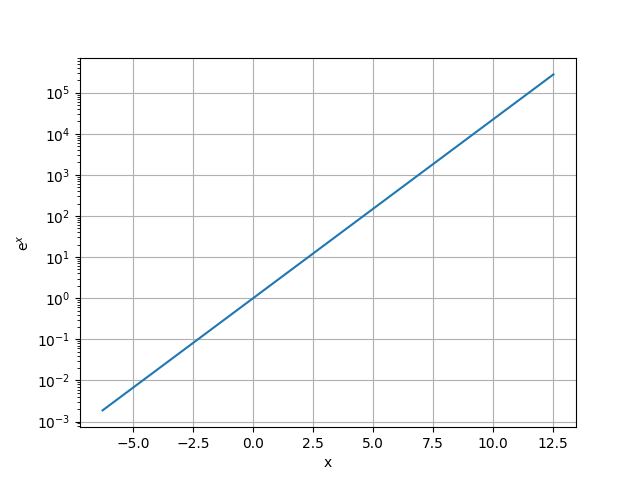
\includegraphics[width=\columnwidth]{expsl.png}
\caption{Semi-log scale plot of e$^{x}$}
\end{figure}
\begin{figure}
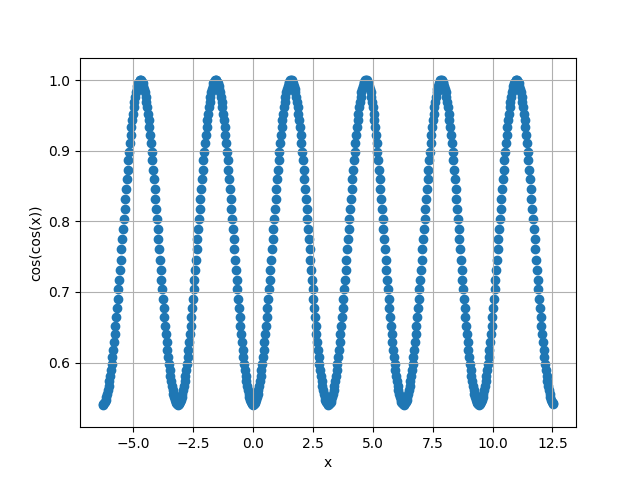
\includegraphics[width=\columnwidth]{coscossl.png}
\caption{Plot of cos(cos(x)) in linear scale}
\end{figure}
\subsection{Expected Fourier Approximation}
Expected output for cos(cos(x)) would be the function itself as it is periodic and has no discontinuity.Where as in case of e$^{x}$ which in non-periodic the output expected would be a periodic part of function from 0 to 2$\pi$ repeating in the domain here in this case \-2$\pi$ to 4$\pi$ it will repeat thrice.See Figure 3 and Figure 4.
\begin{lstlisting}
#expected output by fourier series for coscos(x)
plt.plot(x,cos_arr)
plt.title("Expected fourier approximation for cos(cos(x)) ")
plt.show()
#expected output by fourier series for exp(x)
x3 = np.arange(0,2*np.pi,np.pi/100)
expec_ex = np.array(list(exp(x3))+list(exp(x3))+list(exp(x3)))
plt.plot(x,expec_ex)
plt.title("Expected fourier approximation for e$^{x}$ ")
plt.show()
\end{lstlisting}

\begin{figure}
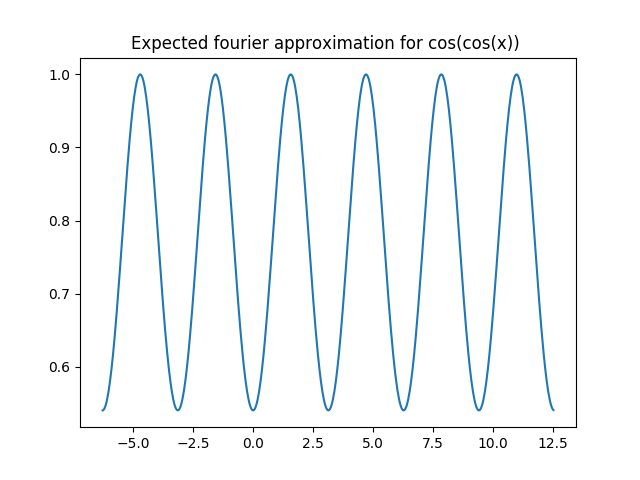
\includegraphics[width=\columnwidth]{expectedcoscos.png}
\caption{Expected Fourier Approximation of cos(cos(x))}
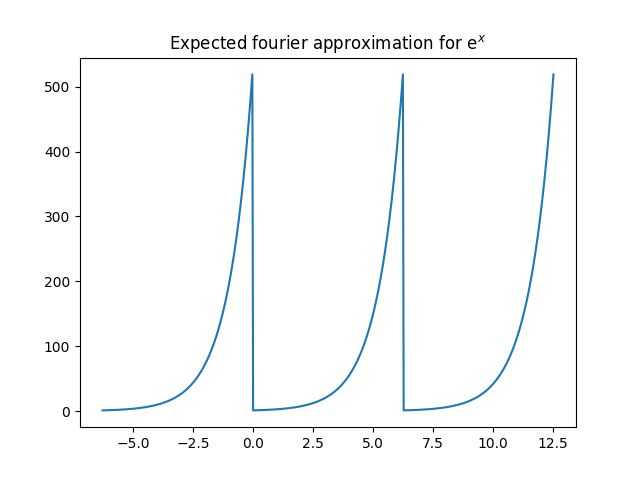
\includegraphics[width=\columnwidth]{expectedex.png}
\caption{Expected Fourier approximation exp(x)}
\end{figure}
\subsection{Obtaining Fourier Coefficients}
First part of this subproblem involves defining the function inside the integral to calculate a\'s and b\'s. And then defining zero vector of size 26 each for an and bn respectively.First element of b will be zero i.e. their index in the vector is the subscript value. Giving in total of fifty\-one  Fourier Coefficients including a$_{o}$. 

\begin{lstlisting}
#defining a function to multiply cos and sine to parameter function. To be used to calculate fourier series
def four_a(x,f,n):
	return f(x)*np.cos(n*x)
def four_b(x,f,n):
	return f(x)*np.sin(n*x)

#creating zero vectors to store fourier coefficients
#An : for a's
#Bn : for b's
An=np.zeros(26)
Bn=np.zeros(26)

\end{lstlisting}
\subsection{Function to compute Fourier Coefficients}
The defined function computes the integral of the defined functions in last code fragment from 0 t0 $\pi$ to compute the a$^{n}$\'s and b$^{n}$\'s.
\begin{lstlisting}
#Defied function calculates and returns fourier coefficients (a's and b's) of the parameter function.

def coeff(f):
	for i in range(26):
		if(i==0):
			An[i] = (quad(four_a,0,2*np.pi,args=(f,i,))[0]/(2*np.pi))#computing integral using quad to canculate a0
		else:
			An[i] = (quad(four_a,0,2*np.pi,args=(f,i,))[0]/(np.pi))#for the rest of the coefficient calculating integral using quad
			Bn[i] = (quad(four_b,0,2*np.pi,args=(f,i,))[0]/(np.pi))
	return An,Bn

\end{lstlisting}

\subsection{Plotting Fourier coefficients of cos(cos(x))}
The function defined in last code fragment accepts function and returns a$^{n}$ and b$^{n}$ in separate arrays.
Passing cos(cos(x)) to the function plotting the obtained coefficients against n in log-log and semi-log scale. See Figure 5 and Figure 6
\begin{lstlisting}
a_coscos,b_coscos = coeff(coscos)

#plotting cos(cos(x)) coefficients on log-log scale
n = np.arange(0,26)
plt.loglog(n,abs(a_coscos),"r+")
plt.loglog(n[1:],abs(b_coscos[1:]),"r+")
plt.legend("a$_{n}$","b$_{n}$")
plt.grid(True)
plt.title("Log-Log plot of cos(cos(x)) coefficients")
plt.show()

#plotting cos(cos(x)) coefficients on semi-log scale
plt.semilogy(n,abs(a_coscos),"r+")
plt.semilogy(n[1:],abs(b_coscos[1:]),"r+")
plt.legend("a$_{n}$","b$_{n}$")
plt.grid(True)
plt.title("Semi-Log plot of cos(cos(x)) coefficients")
plt.show()

\end{lstlisting}
\begin{figure}
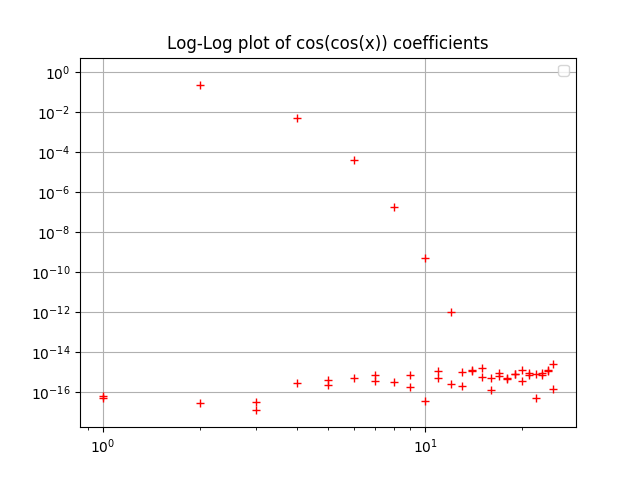
\includegraphics[width=\columnwidth]{coeffllcoscos.png}
\caption{log-log plot of cos(cos(x))}
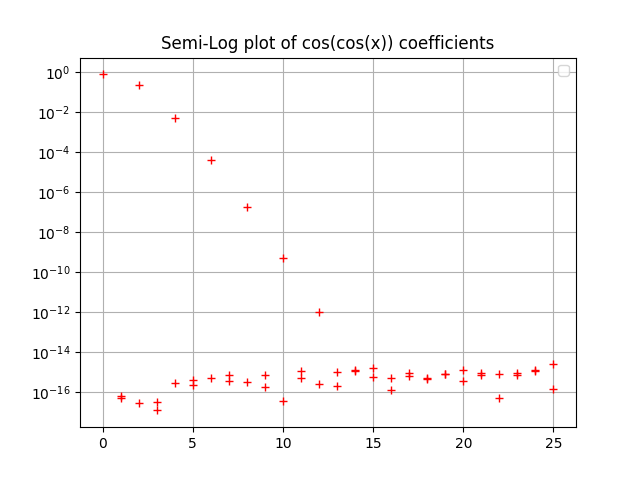
\includegraphics[width=\columnwidth]{coeffslcoscos.png}
\caption{semi-log plot of cos(cos(x))}
\end{figure}
\subsection{Plotting Fourier coefficients of exp(x)}
.Similar to cos(cos(x)) passing e$^{x}$ to the function which returns two arrays which have the values of a$_{0}$ to a$_{25}$ and b$_{1}$ to b$_{25}$ respectively. Plotting the obtained coefficients against n in log-log and semi-log scale. See Figure 7 and Figure 8

\begin{lstlisting}
a_exp,b_exp = coeff(exp)

#plotting Exp(x) coefficients on log-log scale
plt.loglog(n,abs(a_exp),"r+")
plt.loglog(n[1:],abs(b_exp[1:]),"r+")
plt.grid(True)
plt.title("Log-Log plot of e$^{x}$ coefficients")
plt.show()

#plotting Exp(x) coefficients on semi-log scale
plt.semilogy(n,abs(a_exp),"r+")
plt.semilogy(n[1:],abs(b_exp[1:]),"r+")
plt.grid(True)
plt.title("Semi-Log plot of e$^{x}$ coefficients")
plt.show()


\end{lstlisting}
\begin{figure}
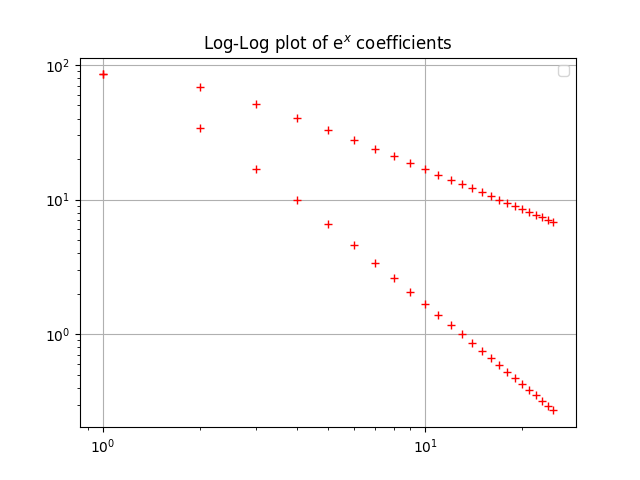
\includegraphics[width=\columnwidth]{coeffllexpx.png}
\caption{Log-Log plot of coefficient of exp(x)}
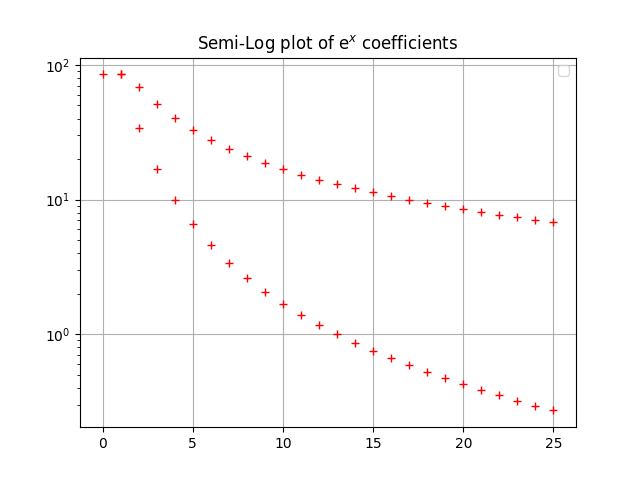
\includegraphics[width=\columnwidth]{coeffslexpx.png}
\caption{Semi-log plot of coefficient of exp(x)}
\end{figure}
\subsection{Answer to problems}
$\bullet$
3) (a) For cos(cos(x)) b$_{n}$ comes out close to zero because cos(cos(x)) is an even function and thus will have coefficient of even part i.e. sin(nx) close to zero.
\linebreak
$\bullet$
3) (b)	e$^(x)$ is not a periodic signal and thus it made periodic by repeating and it is also not a sinusoidal function. Due to discontinuities (emerged due to its repetition) its Fourier series will have high frequency components and we are calculating only 25 terms. Where as cos(cos(x)) is a periodic sinusoidal function and thus its series converges much faster. 
\linebreak
$\bullet$
3) (c) Coefficients of e$^{x}$ i.e. $$ a_{n} ,b_{n} \propto \frac{1}{n^{2}+1} $$
and that is why slope = -log(n$^{2}$+1)*\textbf{constant} $\approx$ -2*log(n)*\textbf{constant} . This shows its linear in log-log scale. Where as coefficients cos(cos(x)) are linearly in semi-log because it is infinitely differentiable and thus its its $$ a^{n},b^{n} \propto \frac{1}{c^{n}} $$
where c is less than 1. So log of the comes out to be n times constant which is negative.
\linebreak
Where as coefficients of cos(cos(x)) i.e. $$ $$
\subsection{Alternative Method : Least Square Approach}
$$ f(x) = \frac{a_{o}}{2} + \sum_{n=1}^{\infty} a_{n}cos(nx) + b_{n}cos(nx) $$
The above equation in matrix form can be represented as
\begin{gather}
 \begin{bmatrix} 1 & cos(x_{1}) & sin(x_{1}) & ... & cos(25x_{1}) & sin(25x_{1}) \\  1 & cos(x_{2}) & sin(x_{2}) & ... & cos(25x_{2}) & sin(25x_{2}) \\ ... & ... & ...& ...& ... \\1 & cos(x_{400}) & sin(x_{400}) & ... & cos(25x_{400}) & sin(25x_{400}) \end{bmatrix}
 \begin{bmatrix}
 a_{0} \\ a_{1} \\ b_{1} \\ ... \\ a_{25} \\ b_{25}
 \end{bmatrix}
 =
  \begin{bmatrix}
 f(x_{1}) \\ f(x_{2}) \\ ... \\ f(x_{400})
   \end{bmatrix}
\end{gather}
We can obtain the R.H.S. of the equation by evaluating functional values at 400 points. Similarly we can obtain cos and sin values at those points to obtain the first matrix. By using Least Squares we can obtain the coefficient matrix. In this assignment we are using in-built least square function of python.
\begin{lstlisting}
x2 = np.linspace(0,2*np.pi,401)
x2=x2[:-1]

def coeff_2(f,x):
	b = f(x)
	A = np.zeros((400,51))
	A[:,0]=1
	for k in range(1,26):
		A[:,2*k-1] = np.cos(k*x)
		A[:,2*k] = np.sin(k*x)
	return linalg.lstsq(A,b)[0]#using least square method built-in python function
\end{lstlisting}

The above defined function takes f(x) and x vector i.e. the points at which we want to evaluate. For this we want points between 0 to 2$\pi$ w ith 400 points.

\subsection{Plotting cos(cos(x)) Fourier coefficients obtained by least squares}

Calling the function defined in last code fragment and plotting the obtained Fourier coefficients against n in log-log scale. Obtained vector with coefficients in not indexed by n. To do so we have to divide a and b in two vectors. Adding a$_{0}$ to a\'s vector named a2\_coscos and remaining even indexes where as odd indexes to b vector named b2\_coscos. See Figure 9.
\begin{lstlisting}
temp = coeff_2(coscos,x2)

#separating a and b coefficients
a2_coscos = np.zeros(26)
a2_coscos[0] = temp[0]
a2_coscos[1:] = temp[1::2]
b2_coscos = temp[2::2]

#plotting log-log of fourier coefficients of cos(cos(x)) by both the methods
plt.loglog(n,abs(a2_coscos),"ro")
plt.loglog(n[1:],abs(b2_coscos),"ro")
plt.loglog(n,abs(a_coscosnew),"gx")
plt.loglog(n[1:],abs(b_coscosnew[1:]),"gx")
plt.grid(True)
plt.legend("coefficients by least square","coefficients by integral")
plt.title("Log-Log plot of cos(cos(x)) coefficients")
plt.show()
\end{lstlisting}
\begin{figure}
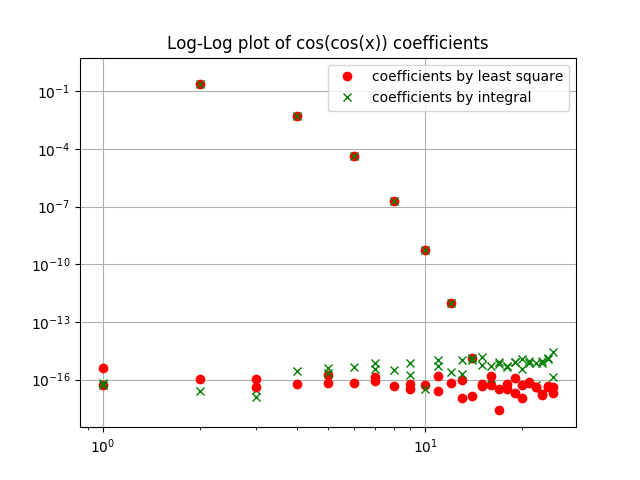
\includegraphics[width=\columnwidth]{coscoscoeffcom.png}
\caption{Green cross are obtained by integral and Red dots by least squares }
\end{figure}
\subsection{Plotting exp(x) Fourier coefficients obtained by least squares}

Calling the function defined in the code fragment one above and plotting the obtained Fourier coefficients against n in log-log scale. Obtained vector with coefficients in not indexed by n. To do so we have to divide a and b in two vectors. Adding a$_{0}$ to a\'s vector named a2\_coscos and remaining even indexes where as odd indexes to b vector named b2\_coscos. See Figure 10.
\begin{lstlisting}
temp = coeff_2(exp,x2)
#separating a and b coefficients
a2_exp = np.zeros(26)
a2_exp[0] = temp[0]https://www.overleaf.com/13818678wvmzjcsgcmmx#
a2_exp[1:] = temp[1::2]
b2_exp = temp[2::2]


#plotting log-log of fourier coefficients of exp(x) by both the methods
plt.loglog(n,abs(a2_exp),"ro")
plt.loglog(n,abs(a_exp),"gx")
plt.loglog(n[1:],abs(b2_exp),"ro")
plt.loglog(n[1:],abs(b_exp[1:]),"gx")
plt.grid(True)
plt.legend("coefficients by least square","coefficients by integral")
plt.title("Log-Log plot of exp(x) coefficients")
plt.show()

\end{lstlisting}
\begin{figure}
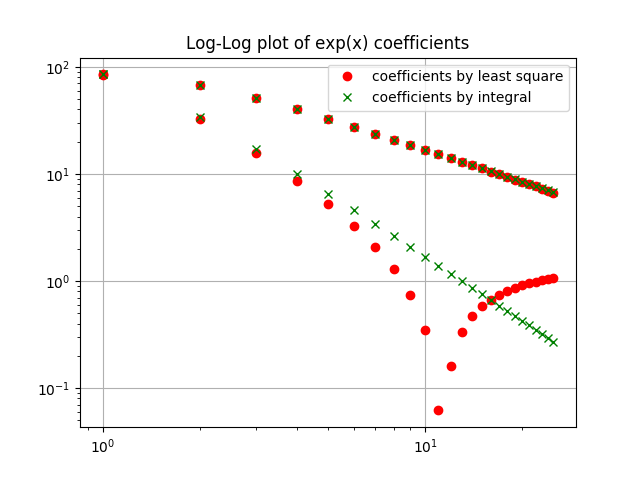
\includegraphics[width=\columnwidth]{expxcoeffcom.png}
\caption{ Green cross are obtained by integral and Red dots by least squares }
\end{figure}

\subsection{Error Measurement Between The two Methods}
For this case we can calculate estimated error i.e. the maximum value of the absolute difference between the coefficients obtained by the two methods.
\subsubsection{Answer to the problem}
$\bullet$
6) No the expected output from both the method is not the same and should not be the same .First method each coefficient is calculated by solving integral which gives correct value.In the second case by least squares since we are taking only 25 coefficients approximation by this method just neglects high frequency components that the signal might have. Hence it gives just an approximate value of the coefficients.

\begin{lstlisting}

a_diff_coscos = a_coscosnew - a2_coscos
b_diff_coscos = b_coscosnew[1:] - b2_coscos


plt.plot(n,a_diff_coscos,"ro")
plt.plot(n[1:],b_diff_coscos,"g+")
plt.show()

a_diff_exp = a_exp - a2_exp
b_diff_exp = b_exp[1:] - b2_exp

plt.plot(n,a_diff_exp,"ro")
plt.plot(n[1:],b_diff_exp,"g+")
plt.show()

print "maximum a diff for e(x) ",max(a_diff_exp)
print "maximum b diff for e(x) ",max(b_diff_exp)
print "maximum a diff for coscos(x) ",max(a_diff_coscos)
print "maximum b diff for coscos(x) ",max(b_diff_coscos)

\end{lstlisting}
The output from the above code gives us,
\begin{lstlisting}

>> maximum a diff for e(x)  1.33273087034
>> maximum b diff for e(x)  0.00349821093269
>> maximum a diff for coscos(x)  8.31811329195e-16
>> maximum b diff for coscos(x)  2.57586713575e-15

\end{lstlisting}
 
From this its clear that the error is extremely small for cos(cos(x)) coefficients . whereas the error is quite significant for e$^{x}$.

\begin{lstlisting}[language=Python ,caption=To generate and plot $1/(1+t^{2})$]
coeff_coscos = []
coeff_coscos.append(a_coscosnew[0])
for i in range(1,26):
	coeff_coscos.append(a_coscosnew[i])
	coeff_coscos.append(b_coscosnew[i])

coeff_exp = []
coeff_exp.append(a_exp[0])
for i in range(1,26):
	coeff_exp.append(a_exp[i])
	coeff_exp.append(b_exp[i])


\end{lstlisting}
\subsection{Approximating the function back by Fourier series}
From the evaluated coefficients we will regenerate the function and plot it.
To obtain the Fourier series sum for convenience merging vector with a\'s and b\'s. In the following order a$^{o}$,a$^{1}$,b$^{1}$,a$^{2}$... and so on.
After converting again substituting this vector in place of coefficient vector in the earlier mentioned matrix equation. After multiplying this to the matrix containing sin(nx) and cos(nx) evaluated and points whose values we desire to obtain. From this matrix multiplication we can obtain reconstructed functional values at 400 points in our case .    
\begin{lstlisting}[language=Python ,caption=To generate and plot $1/(1+t^{2})$]
x3 = np.linspace(0,2*np.pi,401)
x3=x3[:-1]
B = np.zeros((400,51))
B[:,0]=1

#Constructing matrix with sinnx and cosnx 
for k in range(1,26):
	B[:,2*k-1] = np.cos(k*x3)
	B[:,2*k] = np.sin(k*x3)

#multiplying fourier coefficients with sinosoids to approximate the function
re_coscos = np.matmul(B,coeff_coscos)
re_exp = np.matmul(B,coeff_exp)


\end{lstlisting}
The code below is to plot the values obtained above.For cos(cos(x)) and exp(x) see Figure 11 and Figure 12 respectively.
\begin{lstlisting}[language=Python ,caption=To generate and plot $1/(1+t^{2})$]

plt.plot(x3,re_coscos)
plt.title("Approximation of cos(cos(x)) by fourier series")
plt.grid(True)
plt.show()

plt.plot(x3,re_exp)
plt.title("Approximation of e$^{x}$ by fourier series")
plt.grid(True)
plt.show()

\end{lstlisting}
\begin{figure}
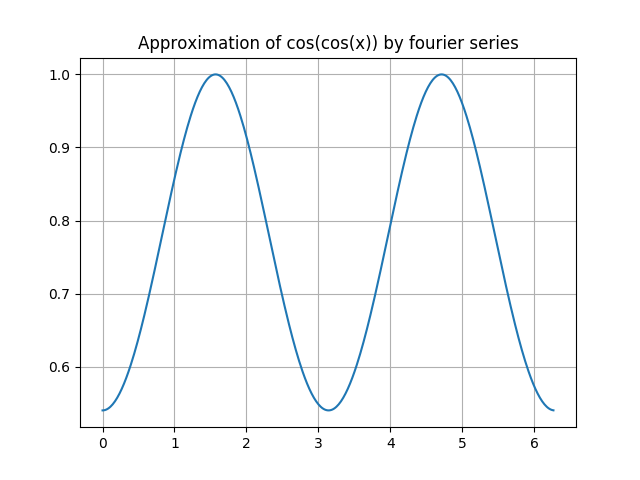
\includegraphics[width=\columnwidth]{approxcoscos.png}
\caption{Approximation of cos(cos(x))}
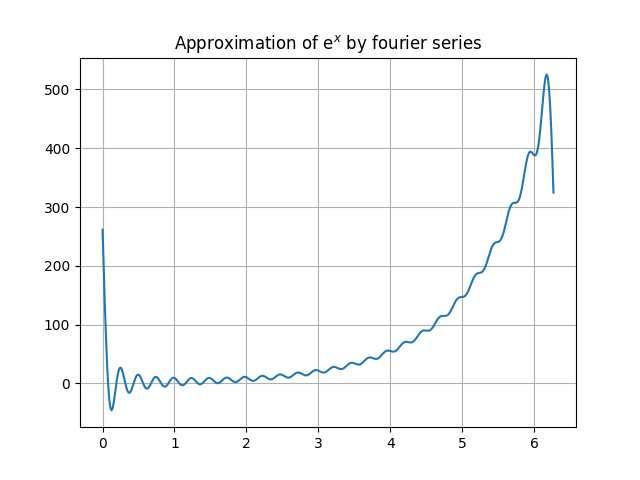
\includegraphics[width=\columnwidth]{approxexpx.png}
\caption{Approximation of exp(x)}
\end{figure}
\subsection{Answer to the problem}
As already mentioned in the answer to last problem. The approximation least squares takes by taking only first 25 terms is to neglect functions higher frequency components. e$^{x}$ has more higher frequency components and can not have an accurate approximation with just 25 coefficients compared to cos(cos(x)) which converges much faster as it has only low frequency components and higher order coefficients tend to zero. The deviation that are at the edges in figure 12 are due to Gibbs phenomena . Since e$^{x}$ is not periodic , for calculating Fourier series the function is repeated from 0 - $2\pi$ and has discontinuity at both the ends.
\end{document}